\documentclass[a4paper, 12pt]{article} % Article starts with section.
% \documentclass[a4paper, 12pt]{report} % Report starts with chapter.

% Edit these for each new project. Make sure to use "\makeatletter" in each new tex file.
% Use the values of \title, \author and \date on a custom title page - Martin Scharrer - https://tex.stackexchange.com/questions/10130/use-the-values-of-title-author-and-date-on-a-custom-title-page - Accessed 12.09.2023
\title{CS4202 Practical 2: Branch Predictor}
\def\subtitle{An analysis of branch prediction strategies}
\author{190018469}
\date{April 2024}

% Language setting
\usepackage[UKenglish]{babel}
\usepackage[utf8]{inputenc}
\usepackage{csquotes}
\usepackage{graphicx} % Required for inserting images
% Set page size and margins
% Replace `letterpaper' with`a4paper' for UK/EU standard size
\usepackage[a4paper,top=2.5cm,bottom=2.5cm,left=3cm,right=3cm,marginparwidth=1.75cm]{geometry}
% ------------------------------ %
% Various useful packages
\usepackage{amsmath}
\usepackage{graphicx}
\usepackage[colorlinks=true, allcolors=blue]{hyperref}
\usepackage{multirow}
\usepackage{float}
% IEEE bibliography setup.
\usepackage[backend=biber, style=ieee, isbn=false,sortcites, maxbibnames=6, minbibnames=1]{biblatex}
\addbibresource{ref.bib} % The references.bib file in which the bibliography used should be.
\usepackage{tabularx} % Tables with dynamic columns.
\usepackage{amssymb}
\usepackage{colortbl}
\usepackage{hyperref}
\usepackage{tikz}
\usepackage[T1]{fontenc} % Extra font options such as small capital (textsc).
\usepackage{lipsum} % Lorem Ipsum Package for placeholder text.
%\usepackage{comment} % Multi-line / Block comments. Doesn't seem to work.
%\usepackage{titlesec}
%\titlespacing*{\subsection}{0pt}{0.5\baselineskip}{0.5\baselineskip}

% Enumerate tag using the alphabet instead of numbers - A.Ellett - https://tex.stackexchange.com/questions/129951/enumerate-tag-using-the-alphabet-instead-of-numbers - Accessed 15.04.2023
\usepackage{enumitem} % Better list customisation

% Subfigures
\usepackage{subfigure}
\usepackage{subcaption}

% Frames for enumerate and itemize.
\usepackage{framed}

%\usepackage{wrapfig} % Wrap figures.
% ------------------------------ %
% Trees
\usepackage[linguistics]{forest}

%\begin{center}
%\begin{forest}
%[Root
%    [L1.1
%        [L2.1\\L2.1E]
%        [L2.2
%            [L3.1\\L3.1E]
%        ]
%    ]
%    [L1.2
%        [L2.3\\L2.3E]
%        [L2.4
%            [L3.2\\L3.2E]
%            [L3.3
%                [L4.1\\L4.1E]
%                [L4.2
%                    [L5.1\\L5.1E]
%                ]
%            ]
%        ]
%    ]
%]
%\end{forest}
%\end{center}



% ------------------------------ %
% Advanced plotting, including from files.
\usepackage{pgfplots}
\pgfplotsset{width=10cm,compat=1.9}

%%% Externalisation does not seem to work.
%% Externalise the figures for faster compilation.
%\usepgfplotslibrary{external}
%\tikzexternalize
%\usetikzlibrary{external}
%\usetikzlibrary[external]
%\tikzexternalize[prefix=tikz/]
% ------------------------------ %
% Code listing - Overleaf - https://www.overleaf.com/learn/latex/Code_listing - Accessed 17.10.2023
% How to make a figure with code? - James - https://tex.stackexchange.com/questions/503533/how-to-make-a-figure-with-code - Accessed 17.10.2023
\usepackage{listings}
\usepackage{xcolor}

\definecolor{codegreen}{rgb}{0,0.6,0}
\definecolor{codegray}{rgb}{0.5,0.5,0.5}
\definecolor{codepurple}{rgb}{0.58,0,0.82}
\definecolor{backcolour}{rgb}{0.95,0.95,0.95}

\lstdefinestyle{mystyle}{
    backgroundcolor=\color{backcolour},   
    commentstyle=\color{codegreen},
    keywordstyle=\color{magenta},
    numberstyle=\tiny\color{codegray},
    stringstyle=\color{codepurple},
    basicstyle=\ttfamily\scriptsize, % Font size (i.e. \scriptsize or \footnotesize)
    breakatwhitespace=false,         
    breaklines=true,                 
    captionpos=b,                    
    keepspaces=true,                 
    numbers=left,                    
    numbersep=5pt,                  
    showspaces=false,                
    showstringspaces=false,
    showtabs=false,                  
    tabsize=2,
    aboveskip=20pt,
}

\lstset{style=mystyle}

%\noindent\begin{minipage}{\linewidth}
%\begin{lstlisting}[caption={captiontext}, label={code:labelname}, frame=single]
%\end{lstlisting}
%\end{minipage}
% ------------------------------ %
% Headers
\usepackage{fancyhdr}
\pagestyle{fancy}
\makeatletter
\lhead{\@title}
\rhead{\@author}
\setlength{\headheight}{15pt}
% ------------------------------ %
% Custom commands
% Guide text: Substitution
\newcommand{\substitution}[1]{[\textit{#1}]}

% Guide text: Optional
\newcommand{\optional}[1]{[#1]}

% Checkmarks and Crossmarks
\usepackage{pifont}
\newcommand{\cmark}{\ding{51}}%
\newcommand{\xmark}{\ding{55}}%
% ------------------------------ %
% Other References:
% set a maximum width and height for an image - Yiannis Lazarides - https://tex.stackexchange.com/questions/47245/set-a-maximum-width-and-height-for-an-image - Accessed 16.04.2023
%\begin{figure}[H]
        %\centering
        %\includegraphics[width=\textwidth, height=0.3\textheight, keepaspectratio]{ImagePath}
        %\caption{captionText}
        %\label{fig:figureName}
%\end{figure}
% ------------------------------ %
% Scrap code
%\usepackage{geometry}
%\geometry{a4paper, total={170mm,257mm}, left=5mm, top=5mm}
\begin{document}
%\begin{titlepage}
    \begin{center}
    \begin{Large}
        \vspace*{1cm}

        \makeatletter
        \textbf{\Huge \@title}

        \vspace{0.5cm}
        \subtitle
            
        \vspace{1.5cm}

        \textbf{\large \@author}

        \vspace{0pt plus 0.75fill}
       
        
\includegraphics[width=0.6\textwidth]{Template/university-of-st-andrews-logo.png}
        
        \vfill
       
        Computer Science\\
        University of St Andrews\\
        \@date
            
    \end{Large}
    \end{center}
\end{titlepage}
%\tableofcontents
\section{Abstract}
% This section should contain a short overview of the practical: 
%   • What were you asked to do?
%   • What did you achieve?
%   • Which parts have you completed and to what extent?
The coursework specification detailed the implementation and analysis of several branch prediction strategies. These included always taken, two-bit, GShare and profiled predictors. The final implementation additionally includes one-bit, global one-bit and global two-bit predictors. Bit predictors, including the GShare predictor, are tested with a table size range from 32 to 16,384 entries. Tests are done on a range of program traces provided with the specification, both using entire files and smaller portions. In summary, the GShare predictor performed best with a large table size for full trace files and two-bit predictors outperformed one-bit predictors.
\section{Implementation Overview}
% Describe the design of your program. Justify the decisions you made.
The simulator implements several predictors that can be run for a given trace file. An overview of each predictor is given in Figure \ref{fig:predictors}. The one-bit, two-bit and global predictors were developed using material from lectures. The GShare predictor was developed using online resources as a guide on the concept, including the original GShare paper \cite{gshare_paper}, a lecture on branch prediction \cite{pittsburg_branch_prediction}, another university assignment \cite{gshare_assignment_edinburgh} and documentation for the Berkeley Out-of-Order Machine's branch prediction \cite{gshare_boom_core}. Running the simulator without a specified trace file will run all trace files in the \texttt{trace-files} folder. Each trace file is run with all possible predictor types and table sizes. After running one configuration, the table size and misprediction rate is exported into a \texttt{csv} file for the trace file and predictor type. These files served as graph data for the graphs in this report.

\begin{figure}[htbp]
    \begin{framed}
        \begin{itemize}
            \item Always Taken: Always predicts a branch to be taken.
            \item One-Bit: Keeps a table of booleans used to predict the outcome of a branch. The program counter address space maps directly to the table.
            \item Two-Bit: Keeps a table of integers used to predict the outcome of a branch. The integer is set from 0 to 3 to represent FSM states (strongly not taken, weakly not taken, weakly taken and strongly taken). The program counter address space maps directly to the table. A diagram of the FSM is shown in Figure \ref{fig:twoBitPredictorImage}.
            \item Global: Uses a bit predictor for each possible outcome of previous branches (taken or not taken). Whether to use one-bit or two-bit predictors is set at initialisation. The outcomes are tracked using a boolean value. This value is used to choose the predictor.
            \item GShare: Uses a long as a global history register for branch outcomes. This is XORed with the program counter address to map into a two-bit predictor table. Bit shifting and setting enable each bit of the long to represent a previous outcome. A diagram is shown in Figure \ref{fig:gShareImage}.
            \item Profiled: Looks at the outcome of each conditional branch in advance and then chooses to take it if it was taken more than it was not taken.
        \end{itemize}
    \end{framed}
    \caption{A textual overview of predictor types implemented}
    \label{fig:predictors}
\end{figure}

\begin{figure}[htbp]
    \centering
    \subfigure[Overview of a two-bit predictor's finite-state machine for a table entry \cite{gshare_boom_core}]{
        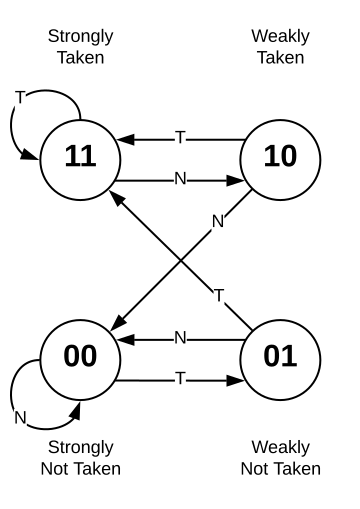
\includegraphics[width=0.425\textwidth, height=0.3\textheight, keepaspectratio]{Images/2BitPredictor.png}
        \label{fig:twoBitPredictorImage}
    }
    \hfill
    \subfigure[Overview of a GShare predictor, showing XOR mapping into a two-bit predictor table \cite{gshare_boom_core}]{
        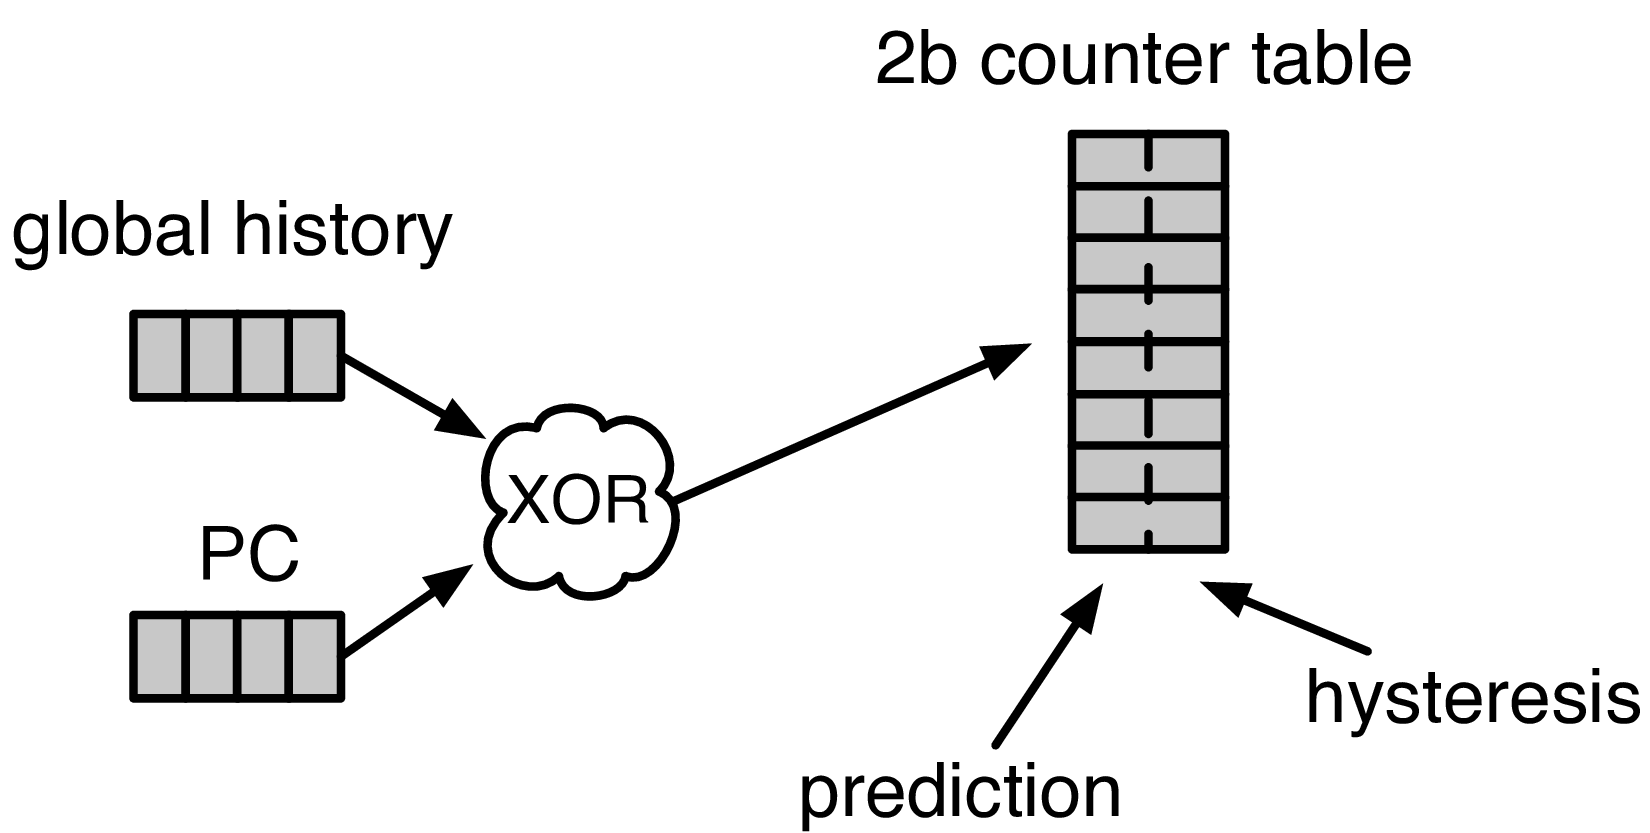
\includegraphics[width=0.525\textwidth, height=0.3\textheight, keepaspectratio]{Images/GSharePredictor.png}
        \label{fig:gShareImage}
    }
    \caption{A visual overview of predictor concepts}
    \label{fig:predictorImages}
\end{figure}

\section{Findings}
\subsection{Full Trace Files}
To begin, the predictors were run for the entirety of each of the trace files provided. Most programs showed the trend that two-bit predictors consistently outperformed one-bit predictors. Furthermore the GShare predictor outperformed both other one- and two-bit predictors, but only at sufficiently high table size. This includes the Cactus BSSN (Figure \ref{fig:cactusbssn}), Exchange 2 (Figure \ref{fig:exchange2}), GCC (Figure \ref{fig:gcc}), POV-Ray (Figure \ref{fig:povray}), XZ (Figure \ref{fig:xz}), WRF (Figure \ref{fig:wrf}) and Leela (Figure \ref{fig:leela}) trace files. Additionally, WRF (Figure \ref{fig:wrf}) has a very small margin between GShare and the other two-bit predictors. The relative downward trend of misprediction rate with increasing table size is likely due to bigger table size resulting in less overlap between program counter addresses. Two addresses are less likely to share the same table entry and as such less likely to interfere with each other's state. The two-bit predictors outperform the one-bit predictors as two-bit predictors introduce hysteresis (a delay in changing prediction) through their additional bit. The additional bit counters the instability of one-bit predictors, which immediately switch their prediction upon a single mistake. This instability presents an issue in branch patterns that frequently alternate between taken and not taken.

% Full trace files (common pattern)
\begin{figure}[htbp]
    \centering
    \ref{leg:traces1} % Put the legend above the plots.

    % GShare (High Predictor Size) < Two-Bit < One-Bit
    \subfigure[Cactus BSSN]{
        \begin{tikzpicture}
            \begin{axis}[
                    %xlabel={Table Size},
                    ylabel={Misprediction Rate (\%)},
                    xmin=32, xmax=65536,
                    %xticklabels={32,64,128,256,512,1K,2K,4K,8K,16K,32K,64K},
                    xticklabels={64,256,1K,4K,16K,64K},
                    ymajorgrids=true,
                    minor tick num=1,yminorgrids=true,
                    grid style=dashed,
                    xmode=log,
                    log basis x=2,
                    width=0.475\textwidth,
                    legend to name=leg:traces1, % Set this plot as reference for the legend.
                ]
                \addplot table[col sep=comma] {../output-data/cactusbssn-OneBitPredictor.csv};
                \addplot table[col sep=comma] {../output-data/cactusbssn-TwoBitPredictor.csv};
                \addplot table[col sep=comma] {../output-data/cactusbssn-GSharePredictor.csv};
                \addplot table[col sep=comma] {../output-data/cactusbssn-GlobalPredictor1.csv};
                \addplot table[col sep=comma] {../output-data/cactusbssn-GlobalPredictor2.csv};
                \addplot table[col sep=comma] {../output-data/cactusbssn-ProfiledPredictor.csv};
                \legend{One-Bit,Two-Bit,GShare,Global (One-Bit),Global (Two-Bit),Profiled}
            \end{axis}
        \end{tikzpicture}
        \label{fig:cactusbssn}
    }
    \hfill
    % GShare (High Predictor Size) < Two-Bit < One-Bit
    \subfigure[Exchange 2]{
        \begin{tikzpicture}
            \begin{axis}[
                    %xlabel={Table Size},
                    %ylabel={Misprediction Rate (\%)},
                    xmin=32, xmax=65536,
                    %xticklabels={32,64,128,256,512,1K,2K,4K,8K,16K,32K,64K},
                    xticklabels={64,256,1K,4K,16K,64K},
                    ymajorgrids=true,
                    minor tick num=1,yminorgrids=true,
                    grid style=dashed,
                    xmode=log,
                    log basis x=2,
                    width=0.475\textwidth,
                ]
                \addplot table[col sep=comma] {../output-data/exchange2-OneBitPredictor.csv};
                \addplot table[col sep=comma] {../output-data/exchange2-TwoBitPredictor.csv};
                \addplot table[col sep=comma] {../output-data/exchange2-GSharePredictor.csv};
                \addplot table[col sep=comma] {../output-data/exchange2-GlobalPredictor1.csv};
                \addplot table[col sep=comma] {../output-data/exchange2-GlobalPredictor2.csv};
                \addplot table[col sep=comma] {../output-data/exchange2-ProfiledPredictor.csv};
            \end{axis}
        \end{tikzpicture}
        \label{fig:exchange2}
    }

    \vspace{\baselineskip} % add some vertical space between the rows

    % GShare (High Predictor Size) < Two-Bit < One-Bit
    \subfigure[GCC]{
        \begin{tikzpicture}
            \begin{axis}[
                    %xlabel={Table Size},
                    ylabel={Misprediction Rate (\%)},
                    xmin=32, xmax=65536,
                    %xticklabels={32,64,128,256,512,1K,2K,4K,8K,16K,32K,64K},
                    xticklabels={64,256,1K,4K,16K,64K},
                    ymajorgrids=true,
                    minor tick num=1,yminorgrids=true,
                    grid style=dashed,
                    xmode=log,
                    log basis x=2,
                    width=0.475\textwidth,
                ]
                \addplot table[col sep=comma] {../output-data/gcc-OneBitPredictor.csv};
                \addplot table[col sep=comma] {../output-data/gcc-TwoBitPredictor.csv};
                \addplot table[col sep=comma] {../output-data/gcc-GSharePredictor.csv};
                \addplot table[col sep=comma] {../output-data/gcc-GlobalPredictor1.csv};
                \addplot table[col sep=comma] {../output-data/gcc-GlobalPredictor2.csv};
                \addplot table[col sep=comma] {../output-data/gcc-ProfiledPredictor.csv};
            \end{axis}
        \end{tikzpicture}
        \label{fig:gcc}
    }
    \hfill
    % GShare (High Predictor Size) < Two-Bit < One-Bit
    \subfigure[POV-Ray]{
        \begin{tikzpicture}
            \begin{axis}[
                    %xlabel={Table Size},
                    %ylabel={Misprediction Rate (\%)},
                    xmin=32, xmax=65536,
                    %xticklabels={32,64,128,256,512,1K,2K,4K,8K,16K,32K,64K},
                    xticklabels={64,256,1K,4K,16K,64K},
                    ymajorgrids=true,
                    minor tick num=1,yminorgrids=true,
                    grid style=dashed,
                    xmode=log,
                    log basis x=2,
                    width=0.475\textwidth,
                ]
                \addplot table[col sep=comma] {../output-data/povray-OneBitPredictor.csv};
                \addplot table[col sep=comma] {../output-data/povray-TwoBitPredictor.csv};
                \addplot table[col sep=comma] {../output-data/povray-GSharePredictor.csv};
                \addplot table[col sep=comma] {../output-data/povray-GlobalPredictor1.csv};
                \addplot table[col sep=comma] {../output-data/povray-GlobalPredictor2.csv};
                \addplot table[col sep=comma] {../output-data/povray-ProfiledPredictor.csv};
            \end{axis}
        \end{tikzpicture}
        \label{fig:povray}
    }

    \vspace{\baselineskip} % add some vertical space between the rows

    % GShare (High Predictor Size) < Two-Bit < One-Bit
    \subfigure[XZ]{
        \begin{tikzpicture}
            \begin{axis}[
                    xlabel={Table Size},
                    ylabel={Misprediction Rate (\%)},
                    xmin=32, xmax=65536,
                    %xticks={32,64,128,256,512,1024,2048,4096,8192,16384,32768,65536},
                    %xticklabels={32,64,128,256,512,1K,2K,4K,8K,16K,32K,64K},
                    xticklabels={64,256,1K,4K,16K,64K},
                    ymajorgrids=true,
                    minor tick num=1,yminorgrids=true,
                    grid style=dashed,
                    xmode=log,
                    log basis x=2,
                    width=0.475\textwidth,
                ]
                \addplot table[col sep=comma] {../output-data/xz-OneBitPredictor.csv};
                \addplot table[col sep=comma] {../output-data/xz-TwoBitPredictor.csv};
                \addplot table[col sep=comma] {../output-data/xz-GSharePredictor.csv};
                \addplot table[col sep=comma] {../output-data/xz-GlobalPredictor1.csv};
                \addplot table[col sep=comma] {../output-data/xz-GlobalPredictor2.csv};
                \addplot table[col sep=comma] {../output-data/xz-ProfiledPredictor.csv};
            \end{axis}
        \end{tikzpicture}
        \label{fig:xz}
    }
    \hfill
    % GShare (High Predictor Size, Just Barely) < Two-Bit < One-Bit
    \subfigure[WRF]{
        \begin{tikzpicture}
            \begin{axis}[
                    xlabel={Table Size},
                    %ylabel={Misprediction Rate (\%)},
                    xmin=32, xmax=65536,
                    %xticklabels={32,64,128,256,512,1K,2K,4K,8K,16K,32K,64K},
                    xticklabels={64,256,1K,4K,16K,64K},
                    ymajorgrids=true,
                    minor tick num=1,yminorgrids=true,
                    grid style=dashed,
                    xmode=log,
                    log basis x=2,
                    width=0.475\textwidth,
                ]
                \addplot table[col sep=comma] {../output-data/wrf-OneBitPredictor.csv};
                \addplot table[col sep=comma] {../output-data/wrf-TwoBitPredictor.csv};
                \addplot table[col sep=comma] {../output-data/wrf-GSharePredictor.csv};
                \addplot table[col sep=comma] {../output-data/wrf-GlobalPredictor1.csv};
                \addplot table[col sep=comma] {../output-data/wrf-GlobalPredictor2.csv};
                \addplot table[col sep=comma] {../output-data/wrf-ProfiledPredictor.csv};
            \end{axis}
        \end{tikzpicture}
        \label{fig:wrf}
    }
    \caption{Branch predictor performance of several program traces exhibiting common behavior}
    \label{fig:traces1}
\end{figure}

\clearpage

Also of note is the finding that the standard one- and two-bit predictors in Leela have a relatively constant performance from a table size of 64 (Figure \ref{fig:leela}). This is likely due to a limited number of program counter addresses used in the address space, making even low table sizes sufficient for maximum predictor performance. While the standard predictors have constant performance, GShare's performance noticeably improves with table size. This is likely due to its increasing ability to use previous branch outcomes to predict future branches.

The only exception to the performance ordering of one-bit, two-bit and GShare is the BWaves trace file (Figures \ref{fig:bwaves} and \ref{fig:bwavesZoomedIn}). Here, GShare performed worse than the two-bit predictors at all table sizes tested and worse than the one-bit predictors below a table size of 256. It is likely that GShare has significant address conflicts below this table size, causing a much higher misprediction rate.

% Full trace files (exceptions)
\begin{figure}[htbp]
    \centering
    % GShare (High Predictor Size) < Two-Bit < One-Bit (Note Constant After 32 bytes)
    \subfigure[Leela]{
        \begin{tikzpicture}
            \begin{axis}[
                    %xlabel={Table Size},
                    ylabel={Misprediction Rate (\%)},
                    xmin=32, xmax=65536,
                    %xticklabels={32,64,128,256,512,1K,2K,4K,8K,16K,32K,64K},
                    xticklabels={64,256,1K,4K,16K,64K},
                    ymajorgrids=true,
                    minor tick num=1,yminorgrids=true,
                    grid style=dashed,
                    xmode=log,
                    log basis x=2,
                    width=0.475\textwidth,
                ]
                \addplot table[col sep=comma] {../output-data/leela-OneBitPredictor.csv};
                \addplot table[col sep=comma] {../output-data/leela-TwoBitPredictor.csv};
                \addplot table[col sep=comma] {../output-data/leela-GSharePredictor.csv};
                \addplot table[col sep=comma] {../output-data/leela-GlobalPredictor1.csv};
                \addplot table[col sep=comma] {../output-data/leela-GlobalPredictor2.csv};
                \addplot table[col sep=comma] {../output-data/leela-ProfiledPredictor.csv};
            \end{axis}
        \end{tikzpicture}
        \label{fig:leela}
    }
    \hfill
    \begin{minipage}[H]{0.45\textwidth}
        \centering
        \vspace{-10\baselineskip} % Adjust the value as needed
        \ref{leg:traces1}
    \end{minipage}

    \vspace{\baselineskip} % add some vertical space between the rows

    % Two-Bit < GShare (Except at low predictor size) < One-Bit
    \subfigure[BWaves]{
        \begin{tikzpicture}
            \begin{axis}[
                    xlabel={Table Size},
                    ylabel={Misprediction Rate (\%)},
                    xmin=32, xmax=65536,
                    %xticklabels={32,64,128,256,512,1K,2K,4K,8K,16K,32K,64K},
                    xticklabels={64,256,1K,4K,16K,64K},
                    ymajorgrids=true,
                    minor tick num=1,yminorgrids=true,
                    grid style=dashed,
                    xmode=log,
                    log basis x=2,
                    width=0.475\textwidth
                ]
                \addplot table[col sep=comma] {../output-data/bwaves-OneBitPredictor.csv};
                \addplot table[col sep=comma] {../output-data/bwaves-TwoBitPredictor.csv};
                \addplot table[col sep=comma] {../output-data/bwaves-GSharePredictor.csv};
                \addplot table[col sep=comma] {../output-data/bwaves-GlobalPredictor1.csv};
                \addplot table[col sep=comma] {../output-data/bwaves-GlobalPredictor2.csv};
                \addplot table[col sep=comma] {../output-data/bwaves-ProfiledPredictor.csv};
            \end{axis}
        \end{tikzpicture}
        \label{fig:bwaves}
    }
    \hfill
    \subfigure[BWaves (Zoomed-In)]{
        \begin{tikzpicture}
            \begin{axis}[
                    xlabel={Table Size},
                    %ylabel={Misprediction Rate (\%)},
                    xmin=32, xmax=65536,
                    %xticklabels={32,64,128,256,512,1K,2K,4K,8K,16K,32K,64K},
                    xticklabels={64,256,1K,4K,16K,64K},
                    ymin=0.2, ymax=0.8,
                    ymajorgrids=true,
                    minor tick num=1,yminorgrids=true,
                    grid style=dashed,
                    xmode=log,
                    log basis x=2,
                    width=0.475\textwidth
                ]
                \addplot table[col sep=comma] {../output-data/bwaves-OneBitPredictor.csv};
                \addplot table[col sep=comma] {../output-data/bwaves-TwoBitPredictor.csv};
                \addplot table[col sep=comma] {../output-data/bwaves-GSharePredictor.csv};
                \addplot table[col sep=comma] {../output-data/bwaves-GlobalPredictor1.csv};
                \addplot table[col sep=comma] {../output-data/bwaves-GlobalPredictor2.csv};
                \addplot table[col sep=comma] {../output-data/bwaves-ProfiledPredictor.csv};
            \end{axis}
        \end{tikzpicture}
        \label{fig:bwavesZoomedIn}
    }
    \caption{Branch predictor performance of several program traces exhibiting unusual behavior}
    \label{fig:traces2}
\end{figure}

The always taken predictor displayed generally very poor performance, except for the WRF program trace (Figure \ref{fig:alwaysTaken}). The misprediction rate of the always taken predictor gives the percentage of conditional branches not taken. This means that the always taken predictor will perform poorly for any programs that do not have a near 100\% rate of conditional branches being taken.

Looking at the profiled predictor in isolation, its misprediction rate for the full trace files ranges from 1.49\% for WRF to 21.33\% for Leela (Figure \ref{fig:profiled}).

Leela's official website states that Leela is a Go playing program that uses a trained neural network. During a game, this neural network is queried to improve prediction from search \cite{leela_website}. The trace file for Leela shows that there are several branches that are reached many times with minor variation. This branch variation matches with how search using a neural network might explore many different options before coming to a conclusion for the next best move.

\begin{figure}[htbp]
    \centering
    \subfigure[Always Taken Predictor Performance]{
        \begin{tikzpicture}
            \begin{axis}[
                    ylabel={Misprediction Rate (\%)},
                    ymajorgrids=true,
                    grid style=dashed,
                    width=0.5\textwidth,
                    xtick={0,...,7},
                    xticklabels={BWaves, Cactus BSSN, Exchange 2, GCC, Leela, POV-Ray, XZ, WRF},
                    nodes near coords,
                    nodes near coords style={font=\scriptsize},
                    nodes near coords align={vertical},
                    xticklabel style={font=\small, rotate=45, anchor=east, align=center},
                    ybar=-0.35cm,
                    ymin=0,
                ]
                \addplot table[col sep=comma, x expr=0] {../output-data/bwaves-AlwaysTakenPredictor.csv};
                \addplot table[col sep=comma, x expr=1] {../output-data/cactusbssn-AlwaysTakenPredictor.csv};
                \addplot table[col sep=comma, x expr=2] {../output-data/exchange2-AlwaysTakenPredictor.csv};
                \addplot table[col sep=comma, x expr=3] {../output-data/gcc-AlwaysTakenPredictor.csv};
                \addplot table[col sep=comma, x expr=4] {../output-data/leela-AlwaysTakenPredictor.csv};
                \addplot table[col sep=comma, x expr=5] {../output-data/povray-AlwaysTakenPredictor.csv};
                \addplot table[col sep=comma, x expr=6] {../output-data/xz-AlwaysTakenPredictor.csv};
                \addplot table[col sep=comma, x expr=7] {../output-data/wrf-AlwaysTakenPredictor.csv};
            \end{axis}
        \end{tikzpicture}
        \label{fig:alwaysTaken}
    }
    \hfill
    \subfigure[Profiled Predictor Performance]{
        \begin{tikzpicture}
            \begin{axis}[
                    %ylabel={Misprediction Rate (\%)},
                    ymajorgrids=true,
                    grid style=dashed,
                    width=0.5\textwidth,
                    xtick={0,...,7},
                    xticklabels={BWaves, Cactus BSSN, Exchange 2, GCC, Leela, POV-Ray, XZ, WRF},
                    nodes near coords,
                    nodes near coords style={font=\scriptsize},
                    nodes near coords align={vertical},
                    xticklabel style={font=\small, rotate=45, anchor=east, align=center},
                    ybar=-0.35cm,
                    ymin=0,
                ]
                \addplot table[col sep=comma, x expr=0] {../output-data/bwaves-ProfiledPredictor.csv};
                \addplot table[col sep=comma, x expr=1] {../output-data/cactusbssn-ProfiledPredictor.csv};
                \addplot table[col sep=comma, x expr=2] {../output-data/exchange2-ProfiledPredictor.csv};
                \addplot table[col sep=comma, x expr=3] {../output-data/gcc-ProfiledPredictor.csv};
                \addplot table[col sep=comma, x expr=4] {../output-data/leela-ProfiledPredictor.csv};
                \addplot table[col sep=comma, x expr=5] {../output-data/povray-ProfiledPredictor.csv};
                \addplot table[col sep=comma, x expr=6] {../output-data/xz-ProfiledPredictor.csv};
                \addplot table[col sep=comma, x expr=7] {../output-data/wrf-ProfiledPredictor.csv};
            \end{axis}
        \end{tikzpicture}
        \label{fig:profiled}
    }
    \caption{Performance of Tableless Predictors}
    \label{fig:tablelessPredictors}
\end{figure}
\subsection{Partial Trace Files}
To look at predictor performance over smaller parts of a trace file, three trace files were broken up into 1,000, 10,000 and 100,000 lines. Cactus BSSN was chosen as it exhibited the most common behaviour identified from the full traces, while Leela and BWaves were chosen as they exhibited behaviour out of the norm. To create the snippets, the code in Listing \ref{code:traceTruncate} was run for each trace file and snippet length.

\noindent\begin{minipage}{\linewidth}
    \begin{lstlisting}[caption={Truncating a trace to 1,000 lines with 1,000,000 offset}, label={code:traceTruncate}, frame=single]
    $ tail -n +1000000 trace.out | head -n 1000 > trace1000_offset.out
\end{lstlisting}
\end{minipage}

Initially, these program trace excerpts used the contents at the start of the full trace file. However, plotting the results of these showed identical results among the different trace files (Cactus BSSN and Leela shown in Figure \ref{fig:badPartials}). This suggests that all the trace files share some initialisation code of the platform from which the trace files were generated. To counter this, each snippet is offset by 1,000,000 lines from the start of the corresponding trace file.

% Bad partials
\begin{figure}[htbp]
    \centering
    \subfigure[Cactus BSSN]{
        \begin{tikzpicture}
            \begin{axis}[
                    %xlabel={Predictor Size (bytes)},
                    %ylabel={Misprediction Rate (\%)},
                    xmin=32, xmax=65536,
                    %xticklabels={32,64,128,256,512,1K,2K,4K,8K,16K,32K,64K},
                    xticklabels={64,256,1K,4K,16K,64K},
                    ymajorgrids=true,
                    grid style=dashed,
                    xmode=log,
                    log basis x=2,
                    width=0.475\textwidth
                ]
                \addplot table[col sep=comma] {../output-data/cactusbssn10000-OneBitPredictor.csv};
                \addplot table[col sep=comma] {../output-data/cactusbssn10000-TwoBitPredictor.csv};
                \addplot table[col sep=comma] {../output-data/cactusbssn10000-GSharePredictor.csv};
                \addplot table[col sep=comma] {../output-data/cactusbssn10000-GlobalPredictor1.csv};
                \addplot table[col sep=comma] {../output-data/cactusbssn10000-GlobalPredictor2.csv};
                \addplot table[col sep=comma] {../output-data/cactusbssn10000-ProfiledPredictor.csv};
            \end{axis}
        \end{tikzpicture}
        \label{fig:badPartials1}
    }
    \hfill
    \subfigure[Leela]{
        \begin{tikzpicture}
            \begin{axis}[
                    %xlabel={Predictor Size (bytes)},
                    %ylabel={Misprediction Rate (\%)},
                    xmin=32, xmax=65536,
                    %xticklabels={32,64,128,256,512,1K,2K,4K,8K,16K,32K,64K},
                    xticklabels={64,256,1K,4K,16K,64K},
                    ymajorgrids=true,
                    grid style=dashed,
                    xmode=log,
                    log basis x=2,
                    width=0.475\textwidth
                ]
                \addplot table[col sep=comma] {../output-data/leela10000-OneBitPredictor.csv};
                \addplot table[col sep=comma] {../output-data/leela10000-TwoBitPredictor.csv};
                \addplot table[col sep=comma] {../output-data/leela10000-GSharePredictor.csv};
                \addplot table[col sep=comma] {../output-data/leela10000-GlobalPredictor1.csv};
                \addplot table[col sep=comma] {../output-data/leela10000-GlobalPredictor2.csv};
                \addplot table[col sep=comma] {../output-data/leela10000-ProfiledPredictor.csv};
            \end{axis}
        \end{tikzpicture}
        \label{fig:badPartials2}
    }
    \caption{Predictor performance for the first 10,000 lines of Cactus BSSN and Leela}
    \label{fig:badPartials}
\end{figure}

% Cactus BSSN Partials Findings:
% GShare fluctuates until 10,000 lines, after which it assumes roughly its final shape. Other predictors reach this by 10,000.

% Cactus BSSN Partials
\begin{figure}[htbp]
    \centering
    \subfigure[1,000 Lines]{
        \begin{tikzpicture}
            \begin{axis}[
                    %xlabel={Predictor Size (bytes)},
                    ylabel={Misprediction Rate (\%)},
                    xmin=32, xmax=65536,
                    %xticklabels={32,64,128,256,512,1K,2K,4K,8K,16K,32K,64K},
                    xticklabels={64,256,1K,4K,16K,64K},
                    ymajorgrids=true,
                    grid style=dashed,
                    xmode=log,
                    log basis x=2,
                    width=0.475\textwidth
                ]
                \addplot table[col sep=comma] {../output-data/cactusbssn1000_offset-OneBitPredictor.csv};
                \addplot table[col sep=comma] {../output-data/cactusbssn1000_offset-TwoBitPredictor.csv};
                \addplot table[col sep=comma] {../output-data/cactusbssn1000_offset-GSharePredictor.csv};
                \addplot table[col sep=comma] {../output-data/cactusbssn1000_offset-GlobalPredictor1.csv};
                \addplot table[col sep=comma] {../output-data/cactusbssn1000_offset-GlobalPredictor2.csv};
                \addplot table[col sep=comma] {../output-data/cactusbssn1000_offset-ProfiledPredictor.csv};
            \end{axis}
        \end{tikzpicture}
        \label{fig:cactusbssnPartials1}
    }
    \hfill
    \subfigure[10,000 Lines]{
        \begin{tikzpicture}
            \begin{axis}[
                    %xlabel={Predictor Size (bytes)},
                    %ylabel={Misprediction Rate (\%)},
                    xmin=32, xmax=65536,
                    %xticklabels={32,64,128,256,512,1K,2K,4K,8K,16K,32K,64K},
                    xticklabels={64,256,1K,4K,16K,64K},
                    ymajorgrids=true,
                    grid style=dashed,
                    xmode=log,
                    log basis x=2,
                    width=0.475\textwidth
                ]
                \addplot table[col sep=comma] {../output-data/cactusbssn10000_offset-OneBitPredictor.csv};
                \addplot table[col sep=comma] {../output-data/cactusbssn10000_offset-TwoBitPredictor.csv};
                \addplot table[col sep=comma] {../output-data/cactusbssn10000_offset-GSharePredictor.csv};
                \addplot table[col sep=comma] {../output-data/cactusbssn10000_offset-GlobalPredictor1.csv};
                \addplot table[col sep=comma] {../output-data/cactusbssn10000_offset-GlobalPredictor2.csv};
                \addplot table[col sep=comma] {../output-data/cactusbssn10000_offset-ProfiledPredictor.csv};
            \end{axis}
        \end{tikzpicture}
        \label{fig:cactusbssnPartials2}
    }

    \vspace{\baselineskip} % add some vertical space between the rows

    \subfigure[100,000 Lines]{
        \begin{tikzpicture}
            \begin{axis}[
                    xlabel={Predictor Size (bytes)},
                    ylabel={Misprediction Rate (\%)},
                    xmin=32, xmax=65536,
                    %xticklabels={32,64,128,256,512,1K,2K,4K,8K,16K,32K,64K},
                    xticklabels={64,256,1K,4K,16K,64K},
                    ymajorgrids=true,
                    grid style=dashed,
                    xmode=log,
                    log basis x=2,
                    width=0.475\textwidth,
                    legend image post style={scale=0.7},
                    legend style={font=\scriptsize},
                ]
                \addplot table[col sep=comma] {../output-data/cactusbssn100000_offset-OneBitPredictor.csv};
                \addplot table[col sep=comma] {../output-data/cactusbssn100000_offset-TwoBitPredictor.csv};
                \addplot table[col sep=comma] {../output-data/cactusbssn100000_offset-GSharePredictor.csv};
                \addplot table[col sep=comma] {../output-data/cactusbssn100000_offset-GlobalPredictor1.csv};
                \addplot table[col sep=comma] {../output-data/cactusbssn100000_offset-GlobalPredictor2.csv};
                \addplot table[col sep=comma] {../output-data/cactusbssn100000_offset-ProfiledPredictor.csv};
                \legend{One-Bit,Two-Bit,GShare,Global (One-Bit),Global (Two-Bit),Profiled}
            \end{axis}
        \end{tikzpicture}
        \label{fig:cactusbssnPartials3}
    }
    \hfill
    \subfigure[Full]{
        \begin{tikzpicture}
            \begin{axis}[
                    xlabel={Predictor Size (bytes)},
                    %ylabel={Misprediction Rate (\%)},
                    xmin=32, xmax=65536,
                    %xticklabels={32,64,128,256,512,1K,2K,4K,8K,16K,32K,64K},
                    xticklabels={64,256,1K,4K,16K,64K},
                    ymajorgrids=true,
                    grid style=dashed,
                    xmode=log,
                    log basis x=2,
                    width=0.475\textwidth
                ]
                \addplot table[col sep=comma] {../output-data/cactusbssn-OneBitPredictor.csv};
                \addplot table[col sep=comma] {../output-data/cactusbssn-TwoBitPredictor.csv};
                \addplot table[col sep=comma] {../output-data/cactusbssn-GSharePredictor.csv};
                \addplot table[col sep=comma] {../output-data/cactusbssn-GlobalPredictor1.csv};
                \addplot table[col sep=comma] {../output-data/cactusbssn-GlobalPredictor2.csv};
                \addplot table[col sep=comma] {../output-data/cactusbssn-ProfiledPredictor.csv};
            \end{axis}
        \end{tikzpicture}
        \label{fig:cactusbssnPartials4}
    }
    \caption{Cactus BSSN run in parts}
    \label{fig:cactusbssnPartials}
\end{figure}

% Leela Partials Findings:
% Normal predictors constant in every case with comparable performance to full trace file. GShare already has best results from 10,000 lines, but only gains its final profile at around 100,000 lines.
% Backs up previous findings. Structure of branches seems to change very little across the runtime of the full program.

% Leela Partials
\begin{figure}[htbp]
    \centering
    \subfigure[1,000 Lines]{
        \begin{tikzpicture}
            \begin{axis}[
                    %xlabel={Predictor Size (bytes)},
                    ylabel={Misprediction Rate (\%)},
                    xmin=32, xmax=65536,
                    %xticklabels={32,64,128,256,512,1K,2K,4K,8K,16K,32K,64K},
                    xticklabels={64,256,1K,4K,16K,64K},
                    ymajorgrids=true,
                    grid style=dashed,
                    xmode=log,
                    log basis x=2,
                    width=0.475\textwidth
                ]
                \addplot table[col sep=comma] {../output-data/leela1000_offset-OneBitPredictor.csv};
                \addplot table[col sep=comma] {../output-data/leela1000_offset-TwoBitPredictor.csv};
                \addplot table[col sep=comma] {../output-data/leela1000_offset-GSharePredictor.csv};
                \addplot table[col sep=comma] {../output-data/leela1000_offset-GlobalPredictor1.csv};
                \addplot table[col sep=comma] {../output-data/leela1000_offset-GlobalPredictor2.csv};
                \addplot table[col sep=comma] {../output-data/leela1000_offset-ProfiledPredictor.csv};
            \end{axis}
        \end{tikzpicture}
        \label{fig:leelaPartials1}
    }
    \hfill
    \subfigure[10,000 Lines]{
        \begin{tikzpicture}
            \begin{axis}[
                    %xlabel={Predictor Size (bytes)},
                    %ylabel={Misprediction Rate (\%)},
                    xmin=32, xmax=65536,
                    %xticklabels={32,64,128,256,512,1K,2K,4K,8K,16K,32K,64K},
                    xticklabels={64,256,1K,4K,16K,64K},
                    ymajorgrids=true,
                    grid style=dashed,
                    xmode=log,
                    log basis x=2,
                    width=0.475\textwidth
                ]
                \addplot table[col sep=comma] {../output-data/leela10000_offset-OneBitPredictor.csv};
                \addplot table[col sep=comma] {../output-data/leela10000_offset-TwoBitPredictor.csv};
                \addplot table[col sep=comma] {../output-data/leela10000_offset-GSharePredictor.csv};
                \addplot table[col sep=comma] {../output-data/leela10000_offset-GlobalPredictor1.csv};
                \addplot table[col sep=comma] {../output-data/leela10000_offset-GlobalPredictor2.csv};
                \addplot table[col sep=comma] {../output-data/leela10000_offset-ProfiledPredictor.csv};
            \end{axis}
        \end{tikzpicture}
        \label{fig:leelaPartials2}
    }

    \vspace{\baselineskip} % add some vertical space between the rows

    \subfigure[100,000 Lines]{
        \begin{tikzpicture}
            \begin{axis}[
                    xlabel={Predictor Size (bytes)},
                    ylabel={Misprediction Rate (\%)},
                    xmin=32, xmax=65536,
                    %xticklabels={32,64,128,256,512,1K,2K,4K,8K,16K,32K,64K},
                    xticklabels={64,256,1K,4K,16K,64K},
                    ymajorgrids=true,
                    grid style=dashed,
                    xmode=log,
                    log basis x=2,
                    width=0.475\textwidth,
                    legend image post style={scale=0.7},
                    legend style={font=\scriptsize},
                ]
                \addplot table[col sep=comma] {../output-data/leela100000_offset-OneBitPredictor.csv};
                \addplot table[col sep=comma] {../output-data/leela100000_offset-TwoBitPredictor.csv};
                \addplot table[col sep=comma] {../output-data/leela100000_offset-GSharePredictor.csv};
                \addplot table[col sep=comma] {../output-data/leela100000_offset-GlobalPredictor1.csv};
                \addplot table[col sep=comma] {../output-data/leela100000_offset-GlobalPredictor2.csv};
                \addplot table[col sep=comma] {../output-data/leela100000_offset-ProfiledPredictor.csv};
                \legend{One-Bit,Two-Bit,GShare,Global (One-Bit),Global (Two-Bit),Profiled}
            \end{axis}
        \end{tikzpicture}
        \label{fig:leelaPartials3}
    }
    \hfill
    \subfigure[Full]{
        \begin{tikzpicture}
            \begin{axis}[
                    xlabel={Predictor Size (bytes)},
                    %ylabel={Misprediction Rate (\%)},
                    xmin=32, xmax=65536,
                    %xticklabels={32,64,128,256,512,1K,2K,4K,8K,16K,32K,64K},
                    xticklabels={64,256,1K,4K,16K,64K},
                    ymajorgrids=true,
                    grid style=dashed,
                    xmode=log,
                    log basis x=2,
                    width=0.475\textwidth
                ]
                \addplot table[col sep=comma] {../output-data/leela-OneBitPredictor.csv};
                \addplot table[col sep=comma] {../output-data/leela-TwoBitPredictor.csv};
                \addplot table[col sep=comma] {../output-data/leela-GSharePredictor.csv};
                \addplot table[col sep=comma] {../output-data/leela-GlobalPredictor1.csv};
                \addplot table[col sep=comma] {../output-data/leela-GlobalPredictor2.csv};
                \addplot table[col sep=comma] {../output-data/leela-ProfiledPredictor.csv};
            \end{axis}
        \end{tikzpicture}
        \label{fig:leelaPartials4}
    }
    \caption{Leela run in parts}
    \label{fig:leelaPartials}
\end{figure}

% BWaves Partials Findings:
% GShare's performance varies widely. Seems to stabilise at around 100,000 lines. (Check:) Of note is that 

% BWaves Partials
\begin{figure}[htbp]
    \centering
    \subfigure[1,000 Lines]{
        \begin{tikzpicture}
            \begin{axis}[
                    %xlabel={Predictor Size (bytes)},
                    ylabel={Misprediction Rate (\%)},
                    xmin=32, xmax=65536,
                    %xticklabels={32,64,128,256,512,1K,2K,4K,8K,16K,32K,64K},
                    xticklabels={64,256,1K,4K,16K,64K},
                    ymajorgrids=true,
                    grid style=dashed,
                    xmode=log,
                    log basis x=2,
                    width=0.472\textwidth
                ]
                \addplot table[col sep=comma] {../output-data/bwaves1000_offset-OneBitPredictor.csv};
                \addplot table[col sep=comma] {../output-data/bwaves1000_offset-TwoBitPredictor.csv};
                \addplot table[col sep=comma] {../output-data/bwaves1000_offset-GSharePredictor.csv};
                \addplot table[col sep=comma] {../output-data/bwaves1000_offset-GlobalPredictor1.csv};
                \addplot table[col sep=comma] {../output-data/bwaves1000_offset-GlobalPredictor2.csv};
                \addplot table[col sep=comma] {../output-data/bwaves1000_offset-ProfiledPredictor.csv};
            \end{axis}
        \end{tikzpicture}
        \label{fig:bwavesPartials1}
    }
    \hfill
    \subfigure[10,000 Lines]{
        \begin{tikzpicture}
            \begin{axis}[
                    %xlabel={Predictor Size (bytes)},
                    %ylabel={Misprediction Rate (\%)},
                    xmin=32, xmax=65536,
                    %xticklabels={32,64,128,256,512,1K,2K,4K,8K,16K,32K,64K},
                    xticklabels={64,256,1K,4K,16K,64K},
                    ymajorgrids=true,
                    grid style=dashed,
                    xmode=log,
                    log basis x=2,
                    width=0.472\textwidth
                ]
                \addplot table[col sep=comma] {../output-data/bwaves10000_offset-OneBitPredictor.csv};
                \addplot table[col sep=comma] {../output-data/bwaves10000_offset-TwoBitPredictor.csv};
                \addplot table[col sep=comma] {../output-data/bwaves10000_offset-GSharePredictor.csv};
                \addplot table[col sep=comma] {../output-data/bwaves10000_offset-GlobalPredictor1.csv};
                \addplot table[col sep=comma] {../output-data/bwaves10000_offset-GlobalPredictor2.csv};
                \addplot table[col sep=comma] {../output-data/bwaves10000_offset-ProfiledPredictor.csv};
            \end{axis}
        \end{tikzpicture}
        \label{fig:bwavesPartials2}
    }

    \vspace{\baselineskip} % add some vertical space between the rows

    \subfigure[100,000 Lines]{
        \begin{tikzpicture}
            \begin{axis}[
                    xlabel={Predictor Size (bytes)},
                    ylabel={Misprediction Rate (\%)},
                    xmin=32, xmax=65536,
                    %xticklabels={32,64,128,256,512,1K,2K,4K,8K,16K,32K,64K},
                    xticklabels={64,256,1K,4K,16K,64K},
                    ymajorgrids=true,
                    grid style=dashed,
                    xmode=log,
                    log basis x=2,
                    width=0.475\textwidth
                ]
                \addplot table[col sep=comma] {../output-data/bwaves100000_offset-OneBitPredictor.csv};
                \addplot table[col sep=comma] {../output-data/bwaves100000_offset-TwoBitPredictor.csv};
                \addplot table[col sep=comma] {../output-data/bwaves100000_offset-GSharePredictor.csv};
                \addplot table[col sep=comma] {../output-data/bwaves100000_offset-GlobalPredictor1.csv};
                \addplot table[col sep=comma] {../output-data/bwaves100000_offset-GlobalPredictor2.csv};
                \addplot table[col sep=comma] {../output-data/bwaves100000_offset-ProfiledPredictor.csv};
            \end{axis}
        \end{tikzpicture}
        \label{fig:bwavesPartials3}
    }
    \hfill
    \subfigure[Full]{
        \begin{tikzpicture}
            \begin{axis}[
                    xlabel={Predictor Size (bytes)},
                    %ylabel={Misprediction Rate (\%)},
                    xmin=32, xmax=65536,
                    %xticklabels={32,64,128,256,512,1K,2K,4K,8K,16K,32K,64K},
                    xticklabels={64,256,1K,4K,16K,64K},
                    ymajorgrids=true,
                    grid style=dashed,
                    xmode=log,
                    log basis x=2,
                    width=0.475\textwidth,
                    legend image post style={scale=0.7},
                    legend style={font=\scriptsize},
                ]
                \addplot table[col sep=comma] {../output-data/bwaves-OneBitPredictor.csv};
                \addplot table[col sep=comma] {../output-data/bwaves-TwoBitPredictor.csv};
                \addplot table[col sep=comma] {../output-data/bwaves-GSharePredictor.csv};
                \addplot table[col sep=comma] {../output-data/bwaves-GlobalPredictor1.csv};
                \addplot table[col sep=comma] {../output-data/bwaves-GlobalPredictor2.csv};
                \addplot table[col sep=comma] {../output-data/bwaves-ProfiledPredictor.csv};
                \legend{One-Bit,Two-Bit,GShare,Global (One-Bit),Global (Two-Bit),Profiled}
            \end{axis}
        \end{tikzpicture}
        \label{fig:bwavesPartials4}
    }
    \caption{BWaves run in parts}
    \label{fig:bwavesPartials}
\end{figure}

% Comment on findings overall.
% Profiled seems to be well suited to small programs or specific parts of larger programs (give examples). It may be worth adapting the profiled approach to predict in blocks of the full code rather than the whole program at once.

% One-Bit < Two-Bit < GShare
%\begin{figure}[H]
%    \centering
%    \begin{tikzpicture}
%    \begin{axis}[
%        xlabel={Predictor Size (bytes)},
%        ylabel={Misprediction Rate (\%)},
%        xmin=32, xmax=65536,
%        xticklabels={32,64,128,256,512,1K,2K,4K,8K,16K,32K,64K},
%        ymajorgrids=true,
%        grid style=dashed,
%        xmode=log,
%        log basis x=2,
%        width=0.75\textwidth,
%        legend pos=north west,
%        legend image post style={scale=0.8},
%        font=\small,
%    ]
%    \addplot table[col sep=comma] {../output-data/bwaves100-OneBitPredictor.csv};
%    \addplot table[col sep=comma] {../output-data/bwaves100-TwoBitPredictor.csv};
%    \addplot table[col sep=comma] {../output-data/bwaves100-GSharePredictor.csv};
%    \addplot table[col sep=comma] {../output-data/bwaves100-GlobalPredictor1.csv};
%    \addplot table[col sep=comma] {../output-data/bwaves100-GlobalPredictor2.csv};
%    \legend{One-Bit,Two-Bit,GShare,Global (One-Bit),Global (Two-Bit)}
%    \end{axis}
%    \end{tikzpicture}
%    \caption{Branch Predictor Performance (BWaves 100)}
%    \label{fig:bwaves100}
%\end{figure}

% Two-Bit < One-Bit < GShare
%\begin{figure}[H]
%    \centering
%    \begin{tikzpicture}
%    \begin{axis}[
%        xlabel={Predictor Size (bytes)},
%        ylabel={Misprediction Rate (\%)},
%        xmin=32, xmax=65536,
%        xticklabels={32,64,128,256,512,1K,2K,4K,8K,16K,32K,64K},
%        ymajorgrids=true,
%        grid style=dashed,
%        xmode=log,
%        log basis x=2,
%        width=0.75\textwidth
%    ]
%    \addplot table[col sep=comma] {../output-data/leela50000-OneBitPredictor.csv};
%    \addplot table[col sep=comma] {../output-data/leela50000-TwoBitPredictor.csv};
%    \addplot table[col sep=comma] {../output-data/leela50000-GSharePredictor.csv};
%    \addplot table[col sep=comma] {../output-data/leela50000-GlobalPredictor1.csv};
%    \addplot table[col sep=comma] {../output-data/leela50000-GlobalPredictor2.csv};
%    \legend{One-Bit,Two-Bit,GShare,Global (One-Bit),Global (Two-Bit)}
%    \end{axis}
%    \end{tikzpicture}
%    \caption{Branch Predictor Performance (Leela 50000)}
%    \label{fig:leela50000}
%\end{figure}
\clearpage
\section{Evaluation}
% Evaluate the success of your program against what you were asked to do.
\section{Conclusion}
% Summarise what you achieved, what you found difficult, and what you would like to do given more time.

%\newpage % Choose one of newpage and clearpage if desired. Clearpage forces any figures to be placed before it.
\clearpage
\printbibliography
%\appendix
\section{Appendix}
\end{document}
% "input" does not include page break wrapping.
% "include" includes page break wrapping.
%TC:ignore - Starts ignoring word count.
%TC:endignore - Ends ignoring word count.